\section{Creation of DeepFakes}\label{sect:creation-of-deepfakes}
Statistical models come in multiple classes with divergent properties.
Two such classes are discriminative and generative models. Generative models
learn the statistical properties of the input domain~\cite[cf.][\nopp{}651\psqq]{Goodfellow.2016}.
For example, they are able to generate unique images of human faces, based on
previously observed ones~\cite{Karras.2019}.

\par
Generative models are thus the focus of techniques for creating DeepFakes. As
this serves as an introduction to the creation of DeepFakes, we limit the scope
to:
% Description of basic network types
\begin{description}[leftmargin=0cm]
    \item[\glspl{ed}] \glspl{ed} consist of at least two networks, \gls{en} and
    \gls{de} (see \cref{subfig:ed}). The \gls{en}-part is trained to extract
    useful features \(\text{En}(x)=e\). This is often done by narrowing
    layer-width towards its center or some other regularization criterion~\cite[cf.][499-505]{Goodfellow.2016}.
    After encoding \(x \rightarrow e\), \(e\) is fed into \gls{de} to arrive at
    the final result \(\text{De}(e)=x_g\). \Glspl{ae} are a special form of
    \gls{ed}, where the network is trained to reproduce its inputs, i.e.\
    \(\text{De}(\text{En}(x))\approx x\).

    \item[\glspl{gan}] \glspl{gan} like \gls{ed} consist of at least two networks,
    \gls{gen} and \gls{disc} (see \cref{subfig:gan}). In a sense, \gls{gen} can
    be interpreted similar to the \gls{de} part of the \gls{ed}. But instead of
    relying on \gls{en} to extract features \(\text{En}(x)=e\), the input
    \(z,\ \text{G}(z)=x_g\) is sampled from a so called prior-distribution
    \(z\sim p_z\), e.g.\ the normal distribution \(p_z=\mathcal{N}(0, 1)\). Then,
    using \(z\), \gls{gen} generates images \(\text{G}(z)=x_g\). \Gls{disc} on
    the other hand tries to discern whether an input is from the original face
    \(x\sim X\) or generated by \gls{gen} \(x_g\). By training \gls{gen} and
    \gls{disc} are then trained alternation, such that \gls{gen} tries to fool
    \gls{disc} into thinking that \(x_g\) is an image from the target and \gls{disc}
    trying to discern correctly between \(x\sim X\) and \(x_g\sim \text{G}(p_z)\).
    That way we are able to generate realistically looking faces similar to that
    of the target~\cite{Goodfellow.2014}.

    \item[\glspl{rnn}] DeepFakes are usually produced in a video setting.
    \Glspl{rnn} are especially built to handle such sequential data and are thus
    a useful extension to \glspl{gan} and \glspl{ed}. At the initial time step,
    \(t=1\), the \gls{rnn} takes input values \(x^{(1)}\) and produces two
    outputs: DeepFake image \(x_g^{(1)}\) and hidden state \(h^{(1)}\). While
    \(x_g^{(1)}\) can be used as the first frame in the video, \(h^{(1)}\) together
    with \(x^{(2)}\) are fed into the model at \(t=2\) to produce the second
    DeepFake frame \(x_g^{(2)}\). This way, the model can preserve knowledge
    about previous frames. More advanced types of \gls{rnn} include \glspl{lstm}
    and \glspl{gru}~\cite[\nopp 404\psqq]{Goodfellow.2016}.
\end{description}
% Figure of basic network types
\begin{figure}[htp]
    \captionsetup[subfigure]{justification=centering}
    \centering
    \begin{minipage}[s][3.3cm]{.23\columnwidth}
        \begin{subfigure}{\columnwidth}
            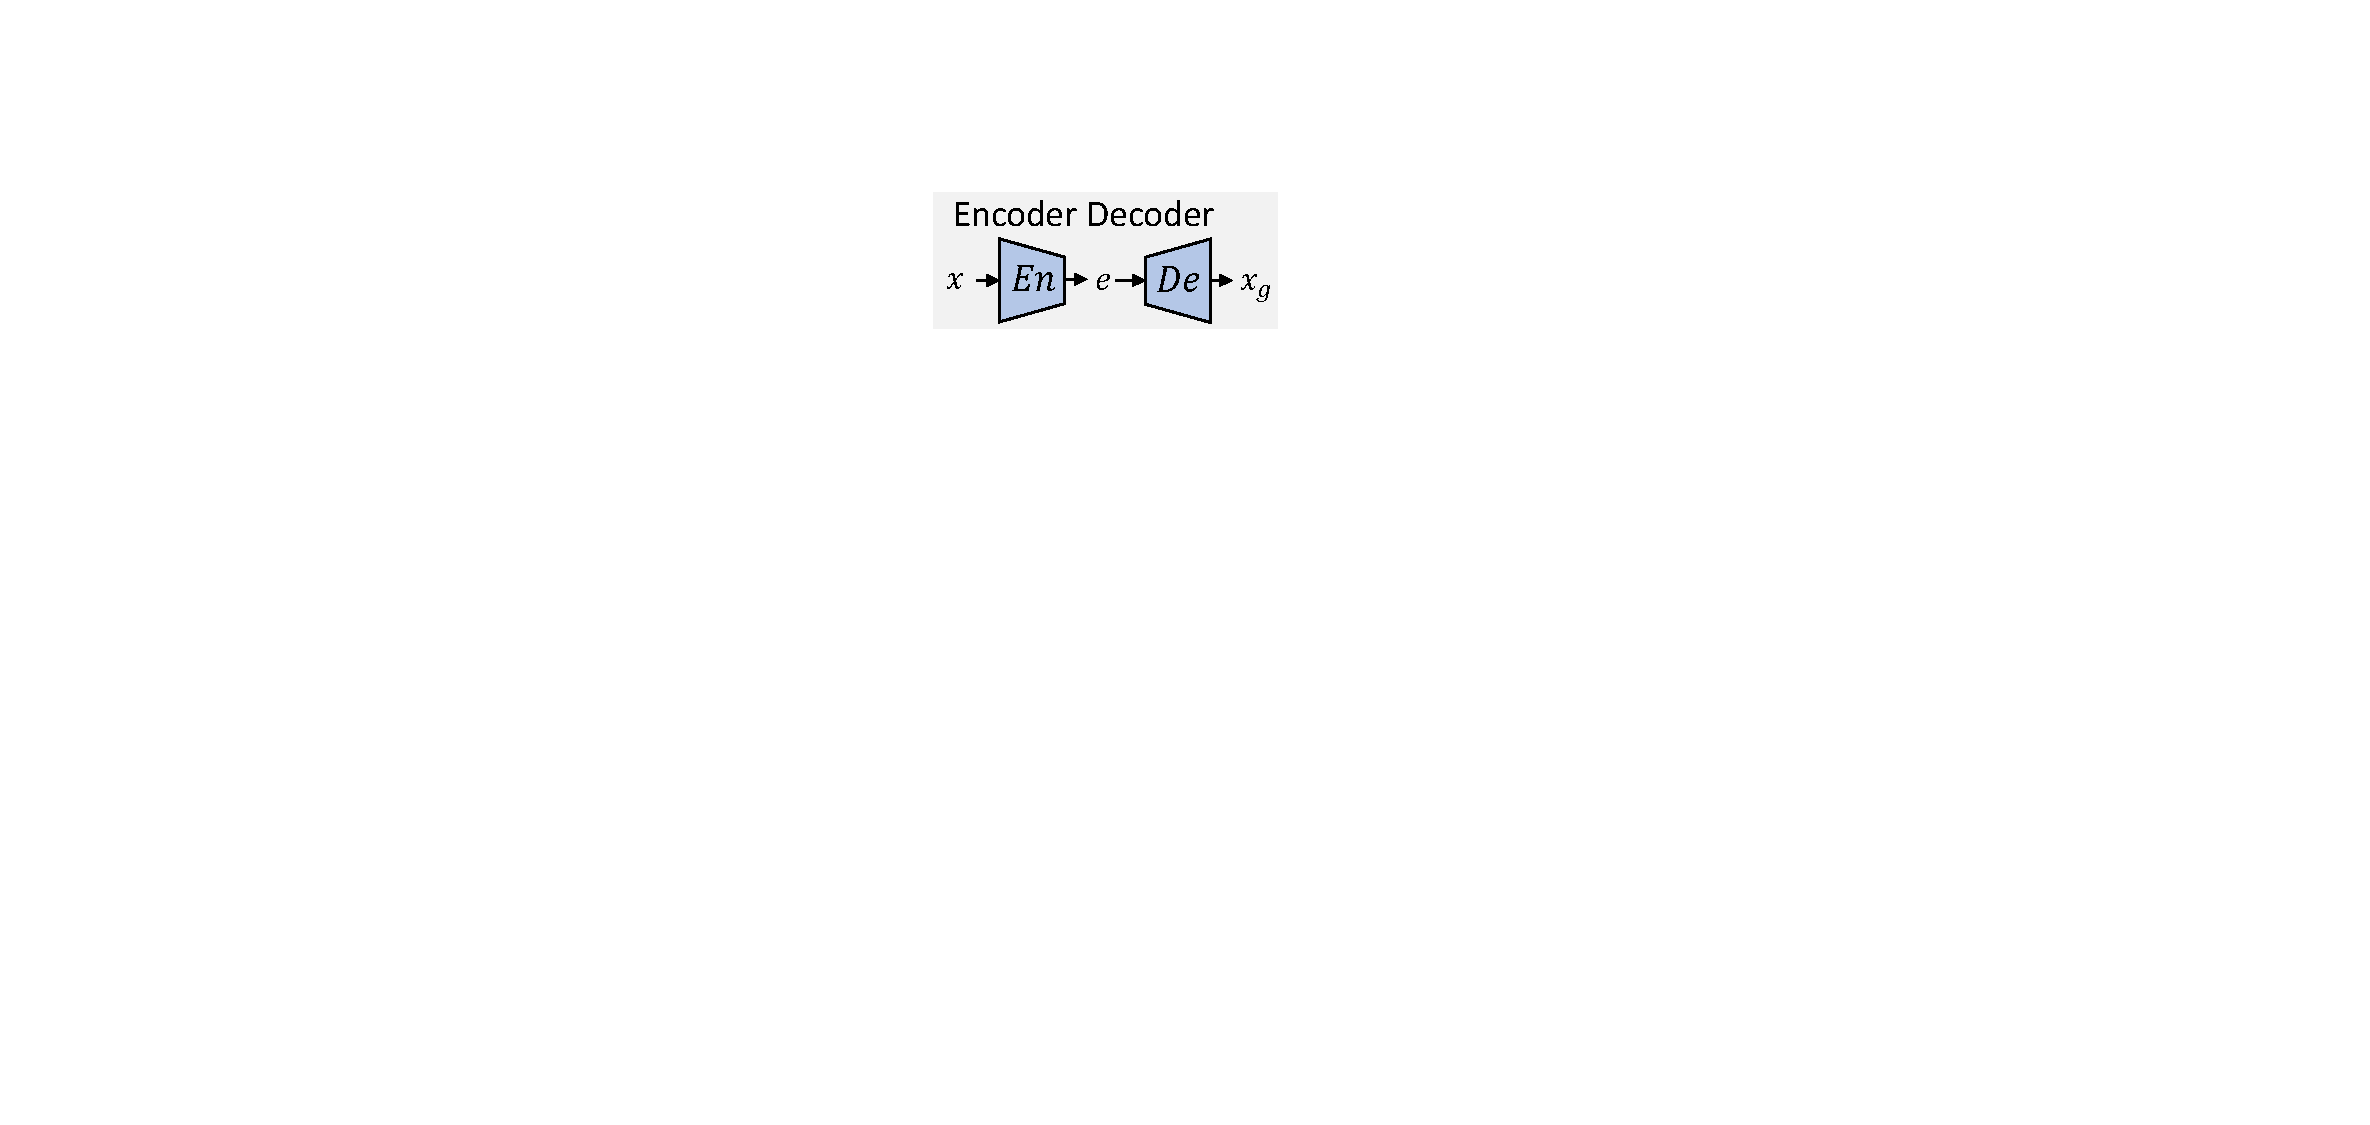
\includegraphics[width=3.3cm]{nns_ed.pdf}
            \caption{}\label{subfig:ed}
        \end{subfigure}
        \vfil
        \begin{subfigure}{\columnwidth}
            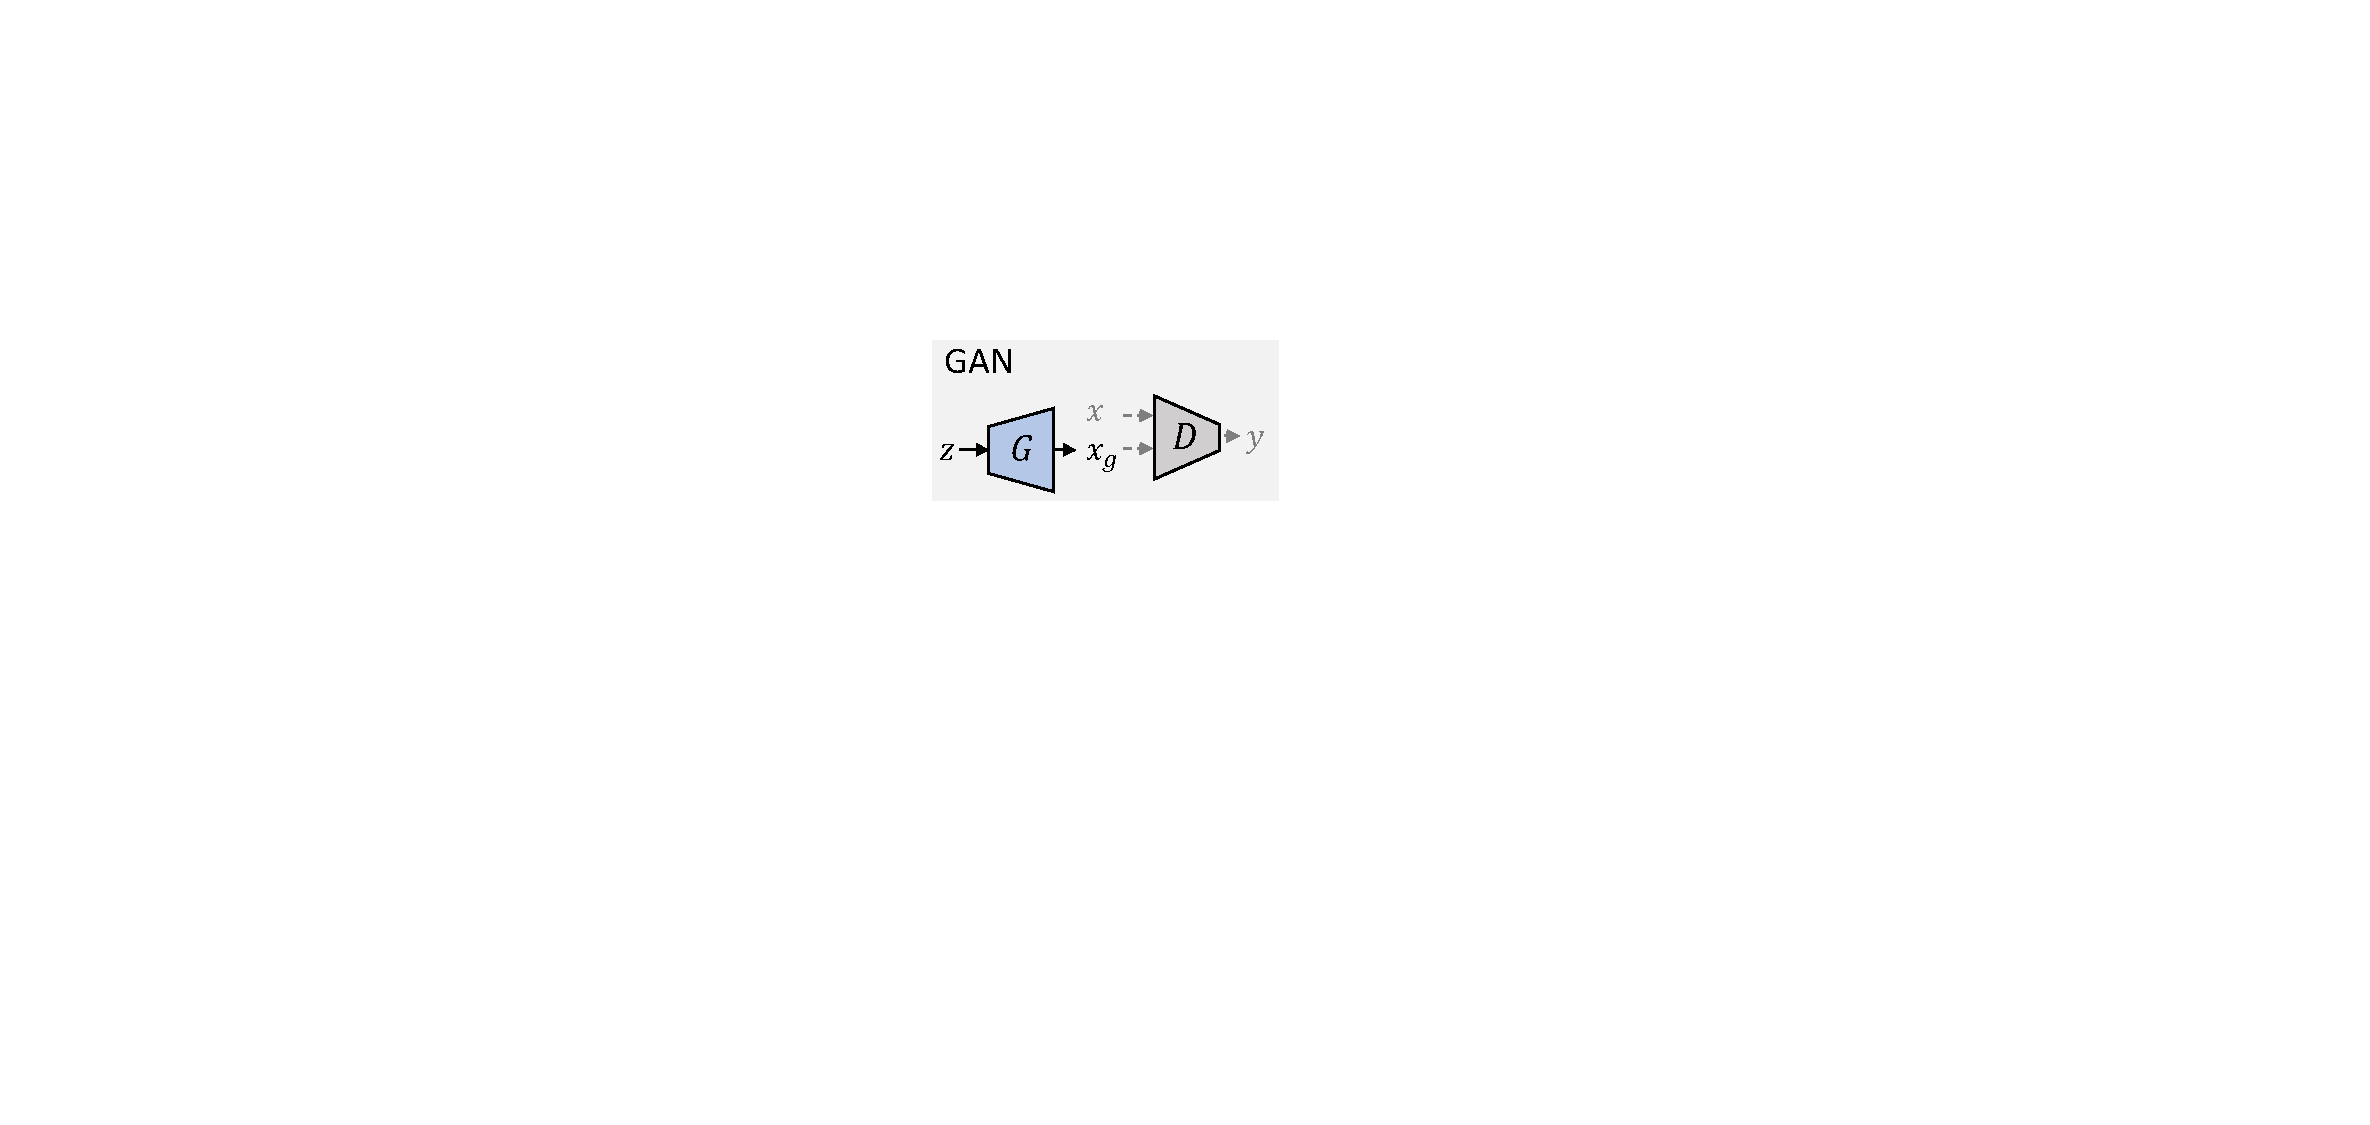
\includegraphics[width=3.3cm]{nns_gan.pdf}
            \caption{}\label{subfig:gan}
        \end{subfigure}
    \end{minipage}
    \begin{subfigure}{.2\columnwidth}
        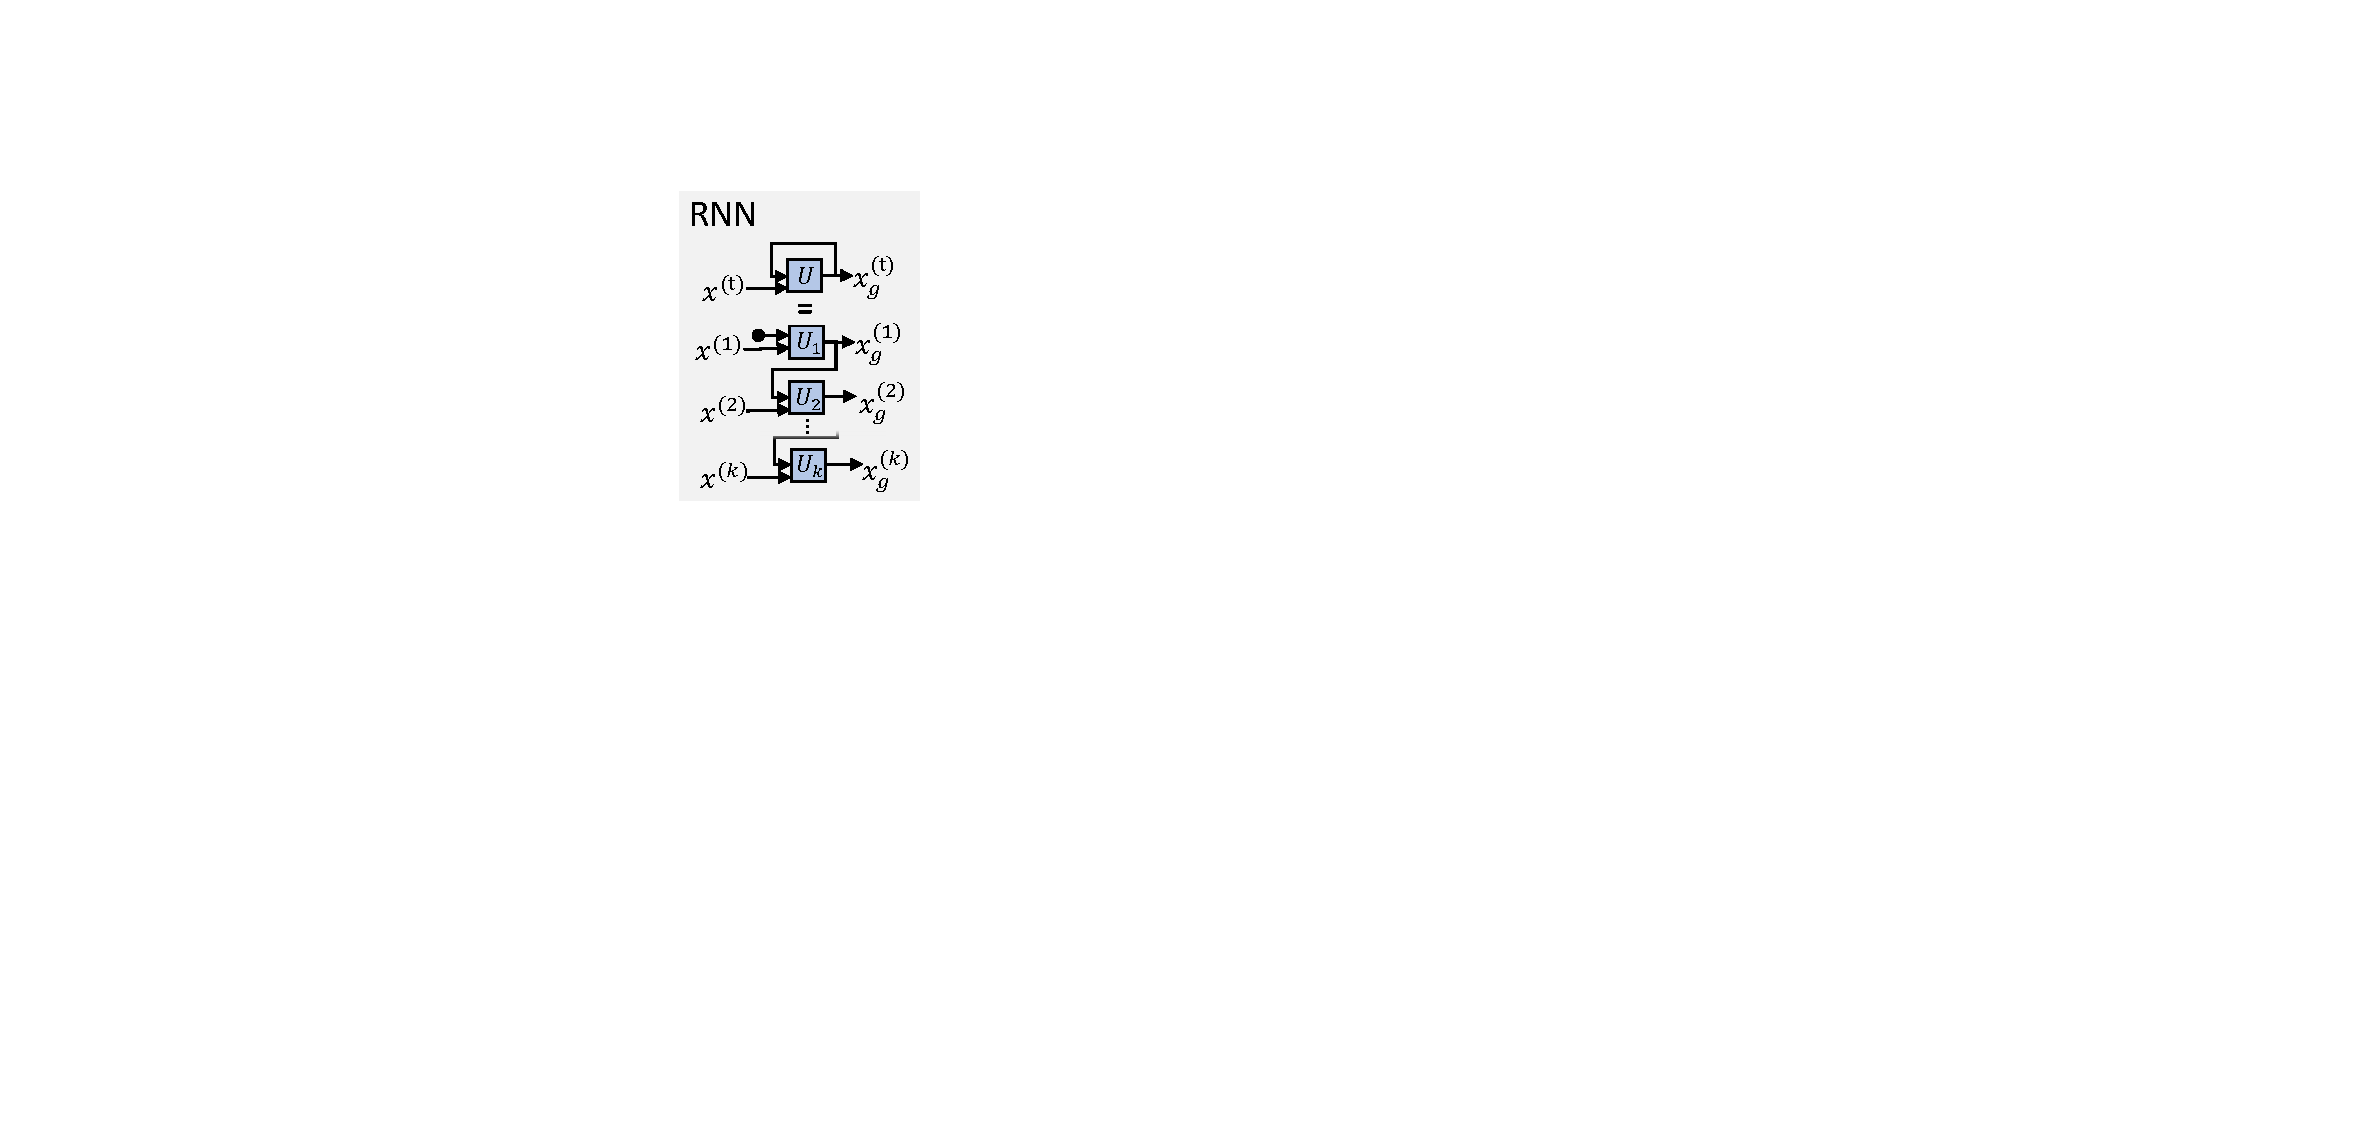
\includegraphics[height=3.7cm]{nns_rnn.pdf}
        \caption{}\label{subfig:rnn}
    \end{subfigure}
    \begin{minipage}[s][3.7cm]{.17\columnwidth}
        \begin{subfigure}{\columnwidth}
            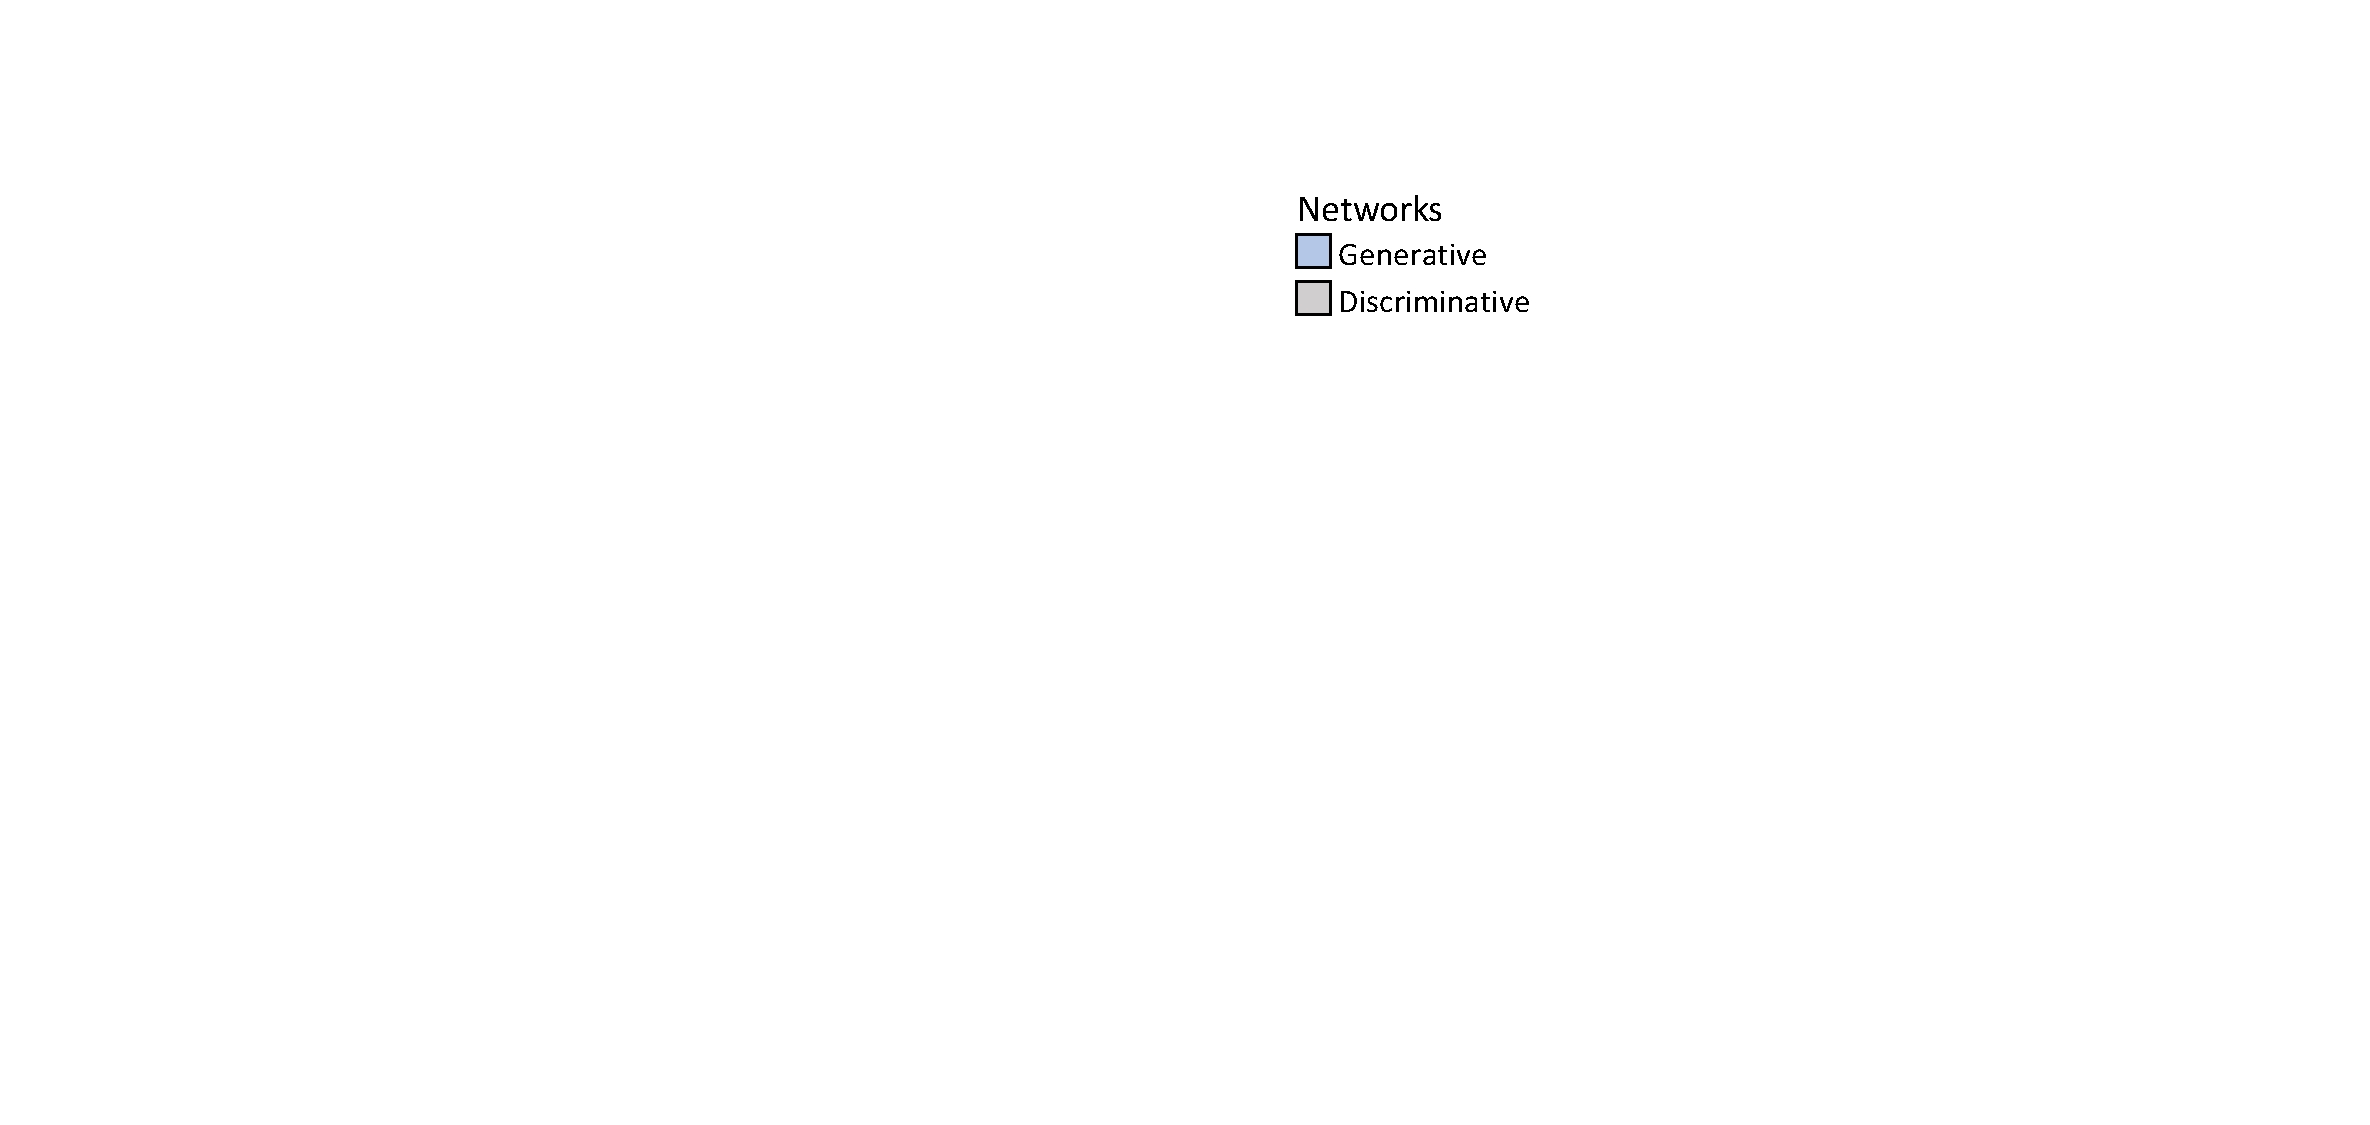
\includegraphics[width=2.5cm]{nns_description.pdf}
        \end{subfigure}\vfil
    \end{minipage}
    \caption{Selection of generative models, adopted from~\cite{Mirsky.2020}}\label{fig:generative-models}
\end{figure}
\subsection{The simplest way to create mimical puppetry}
When trying to create believable mimical puppetry, there are three goals
we try to reach in final image \(x_g\):\todo{explain that \(x_t:target,\ x_s:source\) and so on}
\begin{enumerate}[1.)]
    \item we try to preserve the mimic of \(x_s\) in \(x_g\), s.t.\ \(\text{mimic}(x_s)=\text{mimic}(x_g)\)\label{goal:mimic-perservation}
    \item we try to preserve the identity target \(x_t\) in \(x_g\), s.t.\ \(\text{id}(x_t)=\text{id}(x_g)\)\label{goal:preserve-identity}
    \item we try to generate a realistically looking image\label{goal:increase-realism}
\end{enumerate}
\subsubsection{Generating an image at all}
We can take these goals and construct a model after them. In order to generate
an image we utilize the \gls{ed}-model from \cref{subfig:ed}

\subsubsection{Preserving Mimic}
To tackle the goal~\ref{goal:mimic-perservation}, one must define how to
numerically represent the mimic of a face, \(\text{mimic}(x)=\mathord{?}\).
Two such representations are
\begin{enumerate*}[a.)]
    \item facial landmarks or
    \item \gls{facs}
\end{enumerate*}
For simplicity, only \gls{facs} is considered. A discussion of facial landmarks
can be found in e.g.\ \cite{Ha.2020}

\paragraph*{Facial Action Coding System (FACS)}
The \gls{facs} was introduced in 1978 by \textcite{Ekman.1978}. They grouped
muscle regions of the face to 58 so called \glspl{au} which can be represented
by vectors. A major advantage of \glspl{au} over facial landmarks is that they
are (more or less) invariant (i.e.\ the same expression is encoded similarly)
between faces, head angle and scale~\cite{Pham.2018}.

\par
Following this discussion, \gls{facs} is used. \Glspl{au} might be computed using
a generic \gls{aue}, e.g.\ \cite{Senechal.2015}. The \gls{au}-vectors are then
concatenated to the encoded representation (\(\text{En}(x_t)=e\)) and used in
the \gls{de}-step. To enforce goal~\ref{goal:mimic-perservation}, the difference
in \glspl{au} between final DeepFake \(\text{AUE}(x_g)=a_g\) and driver
\(\text{AUE}(x_s)=a_s\)\todo{decide driver or source} are minimized in training:
\(\min{(\left|a_g-a_s\right|)}\). A visualization of this is given in \cref{fig:gath-aue}.
\begin{figure}[htp]
    \center{}
    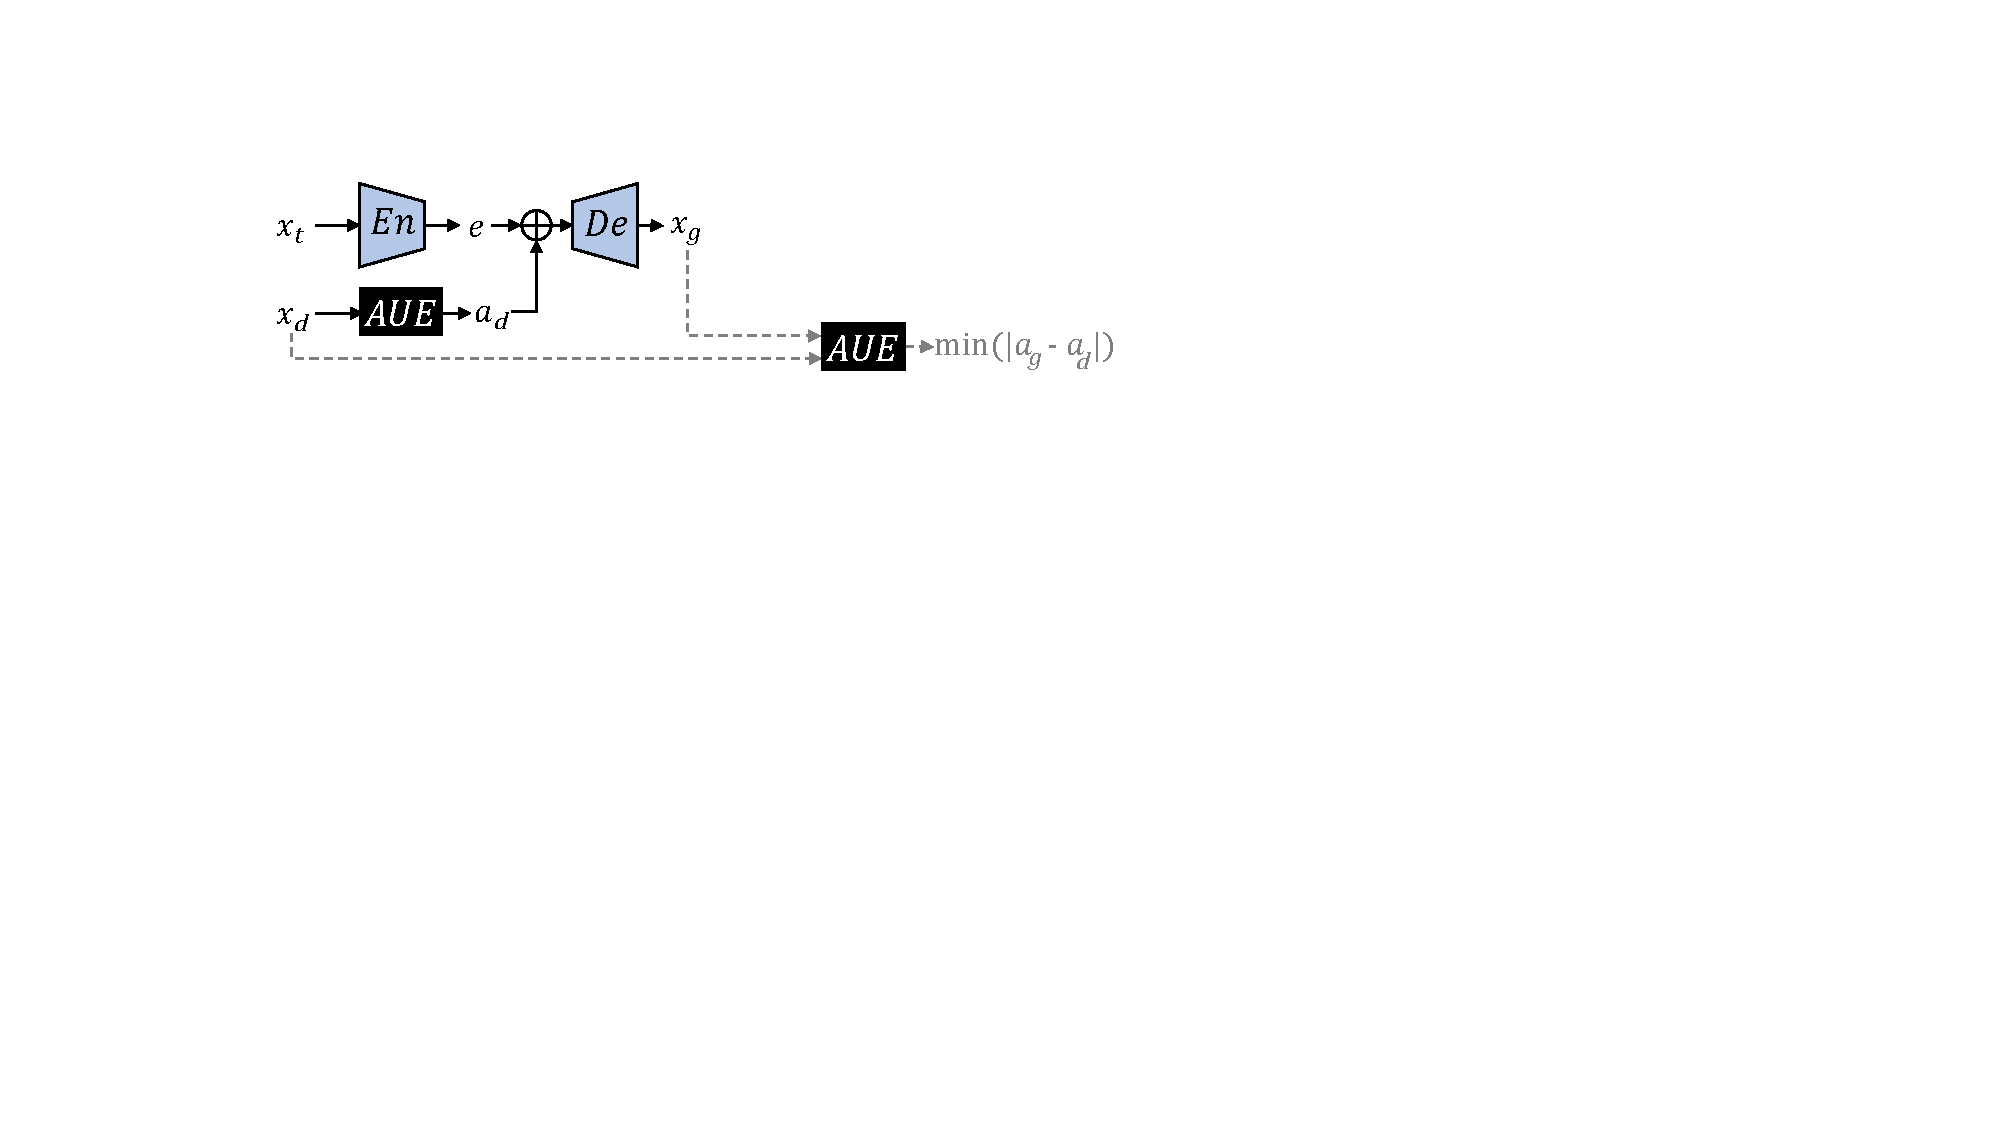
\includegraphics[width=.7\textwidth]{gath_aue.pdf}
    \caption{\gls{ed}-architecture enriched with \glspl{au}, where \(\bigoplus\)
    denotes concatenation. Grey paths are used solely in training, inspired
    by~\cite{Mirsky.2020, Pham.2018}}\label{fig:gath-aue}
\end{figure}

\subsubsection{Preserving Identity}
Training the model on preserving the identity of the target requires a training
set of known targets, e.g.\ \cite{Chen.2015,Cao.2014,Tarres.2011} consisting of 
about 2000 identities~\cite{Pham.2018}. One can then learn an image classifier
\(I\), e.g.\ MobileNet~\cite{Howard.2017} (for its simplicity and speed) to
assign the correct identity to a given image. Once the classifier \(I\)
converges, it can be added to the training procedure of the model, minimizing
the cross-entropy identity loss \(\mathcal{L}_{id}\) (see \cref{eq:identity-loss}).
A visualization of this is given in \cref{fig:gath-aue-id}.
\begin{figure}[htp]
    \center{}
    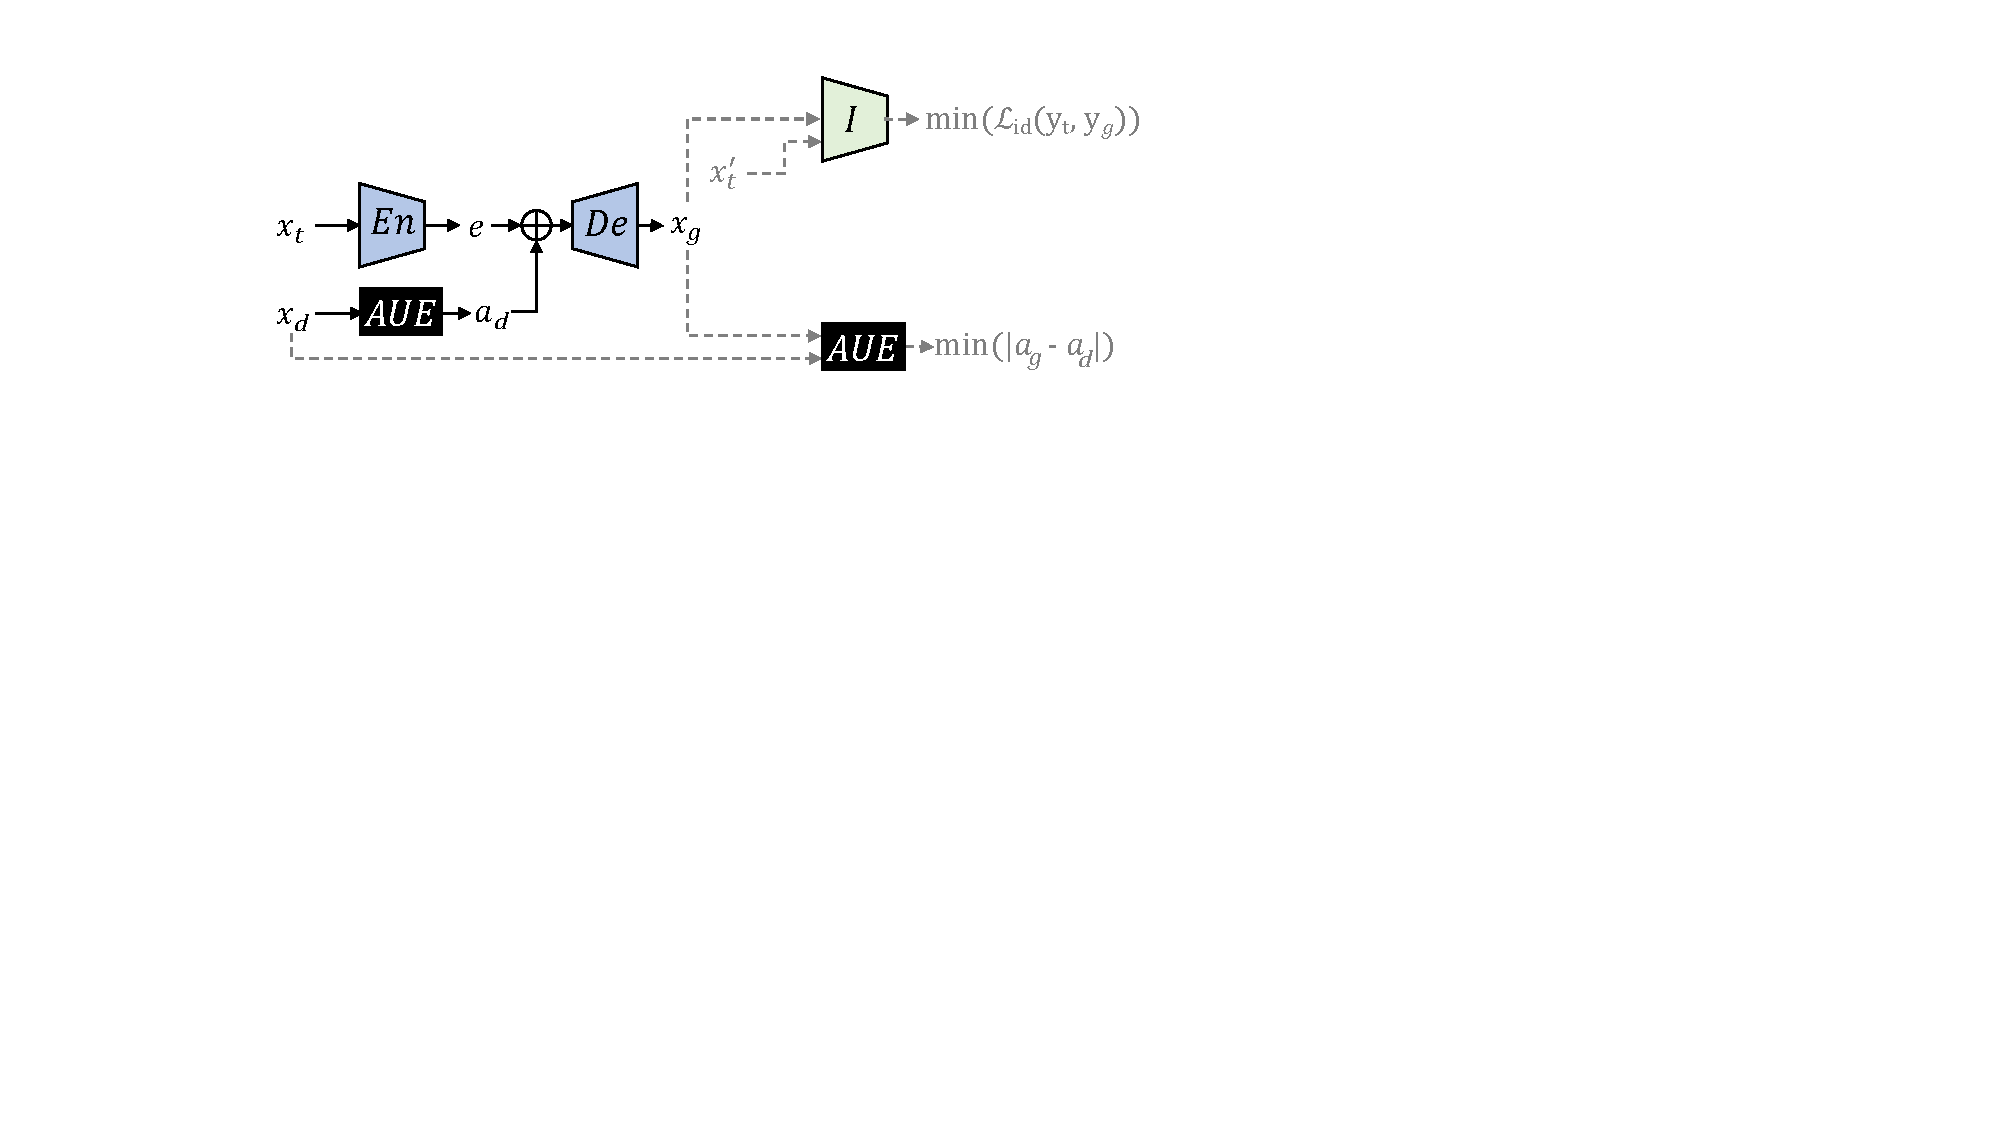
\includegraphics[width=.7\textwidth]{gath_aue_id.pdf}
    \caption{\gls{ed}-architecture enriched with \glspl{au} and an identity
    constraint, where \(\bigoplus\) denotes concatenation, \(x'_t\) is a randomly
    chosen image with identity of the target \(t\). Grey paths are used solely
    in training, inspired by~\cite{Mirsky.2020, Pham.2018}}\label{fig:gath-aue-id}
\end{figure}

\subsubsection{Increase Realism}
Finally to increase realism (goal~\ref{goal:increase-realism}), a \gls{gan}-inspired
discriminator \gls{disc} (see \cref{subfig:gan}) is adopted.
\begin{figure}[htp]
    \center{}
    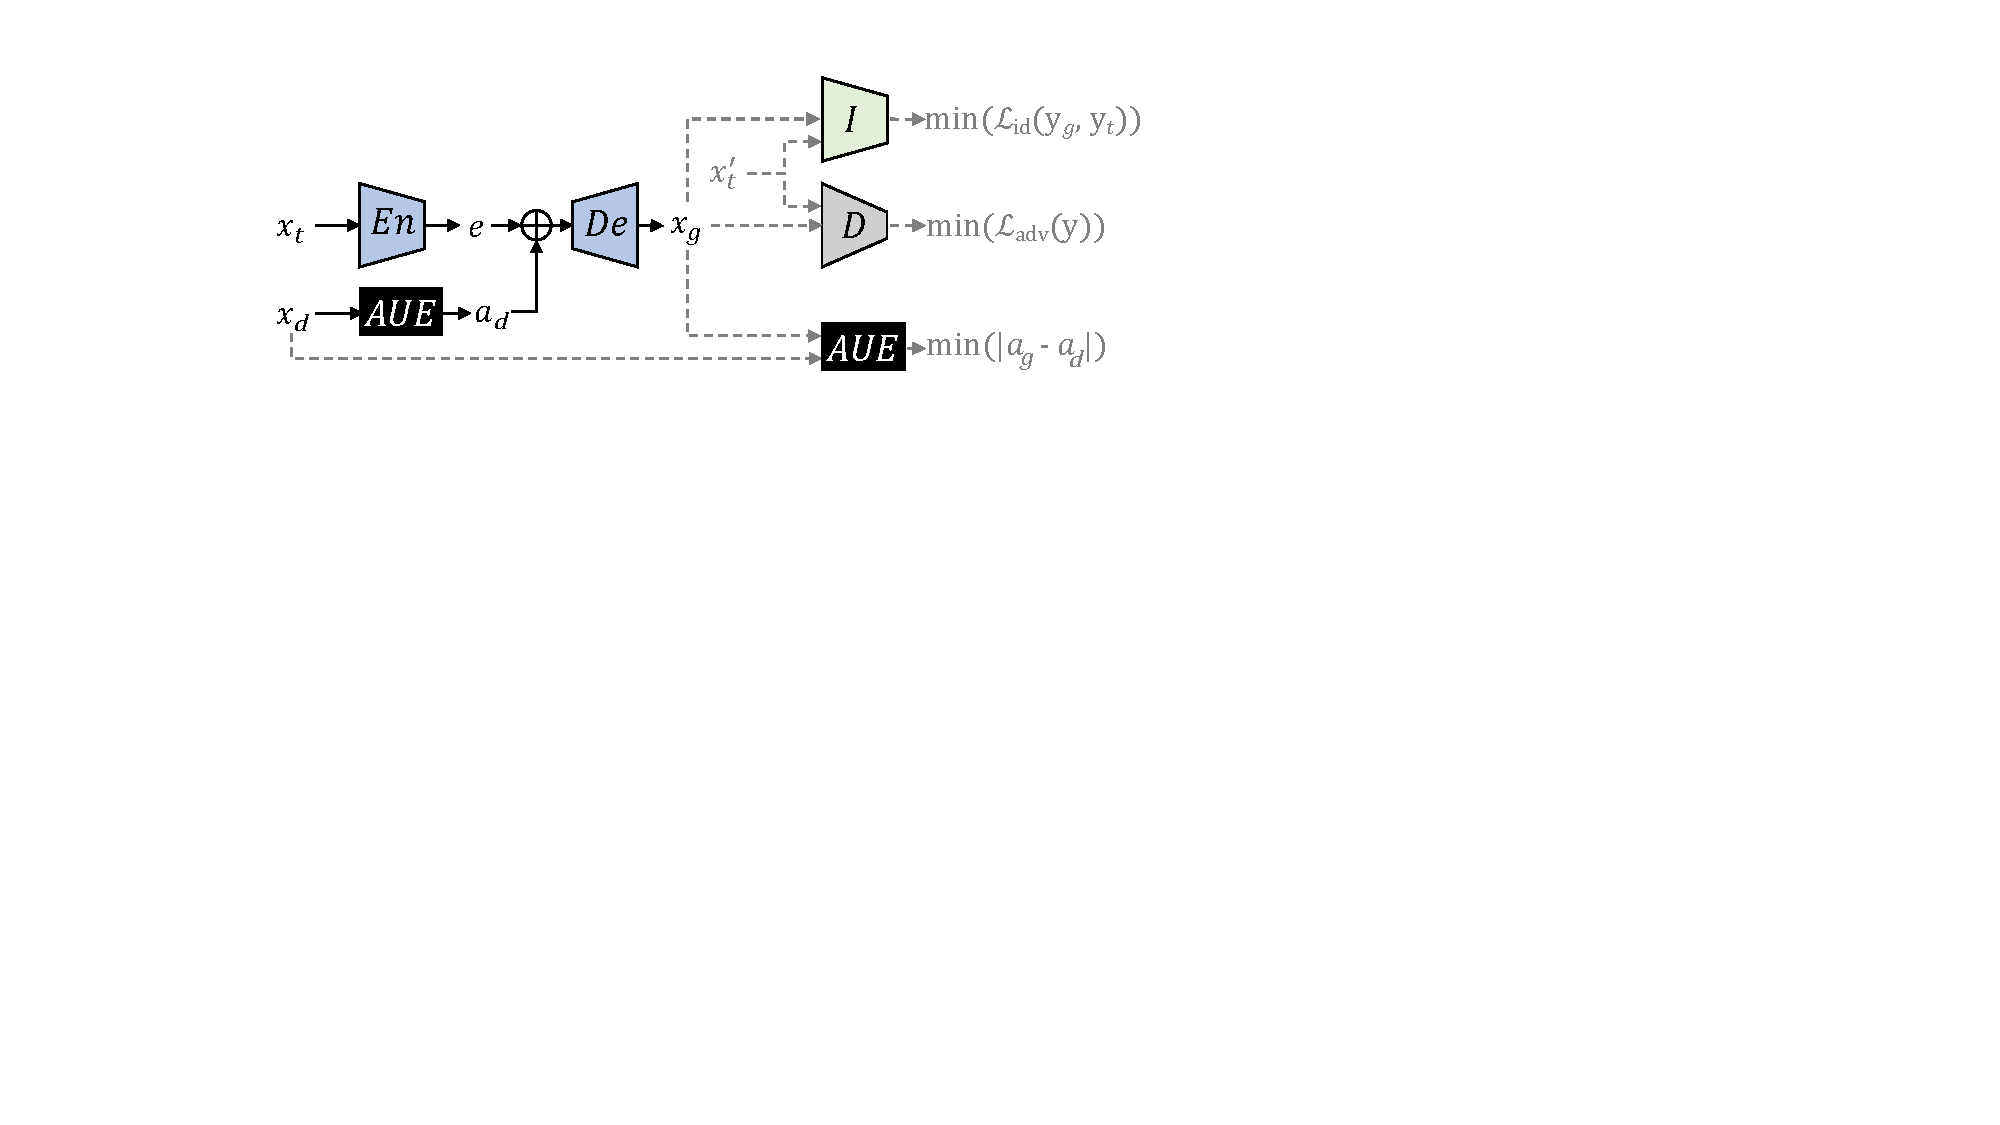
\includegraphics[width=.7\textwidth]{gath_aue_id_disc.pdf}
    \caption{\gls{ed}-architecture enriched with \glspl{au}, an identity
    and an realism constraint, where \(\bigoplus\) denotes concatenation,
    \(x'_t\) is a randomly chosen image with identity of the target \(t\). Grey
    paths are used solely in training, inspired by~\cite{Mirsky.2020, Pham.2018}}\label{fig:gath-aue-id-disc}
\end{figure}

\subsection{The simplest way to create Face Swaps}